\section{Punto de Vista de Realización de Servicio}

Este punto de vista visualiza como por los procesos o componentes de aplicación se realizan los servicios de negocio, evidenciando el puente entre el punto de vista de producto del negocio y la vista de procesos del negocio. Como su nombre lo indica y se observa en el meta-modelo, en este punto de vista se deben identificar los elementos claves para realizar el servicio que ofrece la compañía, es
un tipo de resumen de los elementos generales y que se deben resaltar para comprender en su totalidad el servicio. En este punto de vista el elemento por el cual se debe iniciar el diseño, es el servicio de negocio, de él se derivan los procesos principales y los objetos de negocio asociados al
servicio; teniendo claro que los procesos de negocio se soportan con servicios de aplicación y componentes de aplicación, mientras que los objetos de negocio se realizan con objetos de aplicación. Los elementos que rodean los servicios, se utilizan para hacer claridad en los roles, actores y colaboraciones principales que intervienen en la realización de los procesos.

\subsection{Modelo de Realización de Servicio}
\begin{figure}[h!]
	\centering
	\includegraphics[width=1\linewidth]{imgs/modelo/RealServicio}
	\caption{Modelo Realización de Servicio}
\end{figure}

El punto de vista de realización del servicio muestra los procesos de negocio de la arquitectura: realización de la evaluación, consolidación de la información y análisis de resultados asignados a componentes de aplicación que serán de soporte para dichos proceso. Los procesos de negocio son realizados de forma secuencial y la realización de todos proveen los servicios de negocio definidos.

Este punto de vista cuenta con una gran y amplia serie de elementos que facilitan este proceso, iniciando por el actor en cuestión, con su rol y la colaboración que implica, posteriormente, se centra en el proceso servicio y evento que involucra, teniendo en cuenta también componentes e interfaces.


\subsection{Caso  de Realización de Servicio}
\begin{figure}[h!]
	\centering
	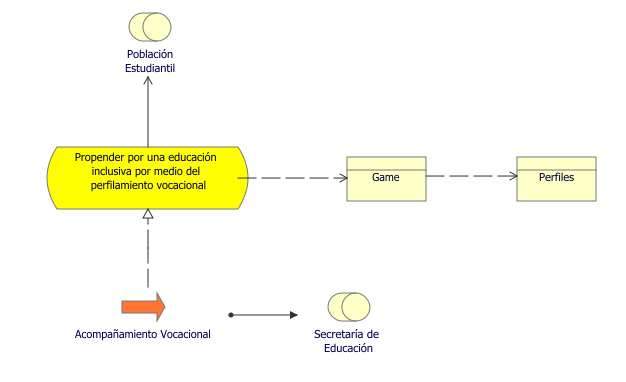
\includegraphics[width=1.05\linewidth]{imgs/caso/RealizaServicio}
	\caption{Caso Realización de Servicio}
\end{figure}

El punto de vista de realización de requerimientos de la parte tecnológica se realiza la vinculación de la información de la base de datos con los procesos de negocio, en busca de un ruta para abstraer nuevos elementos. En el caso del proyecto Tu-Perfil, se destaca el servicio principal de propender por una educación inclusiva por medio del perfilamiento vocacional que a su vez está dirigida al actor de la población estudiantil y a la secretaría de educación nacional a través del proceso de negocio principal llamado acompañamiento vocacional, posteriormente se encuentran los objetos Game o juego y el objeto de los Perfiles. De esta manera se construye el punto de vista de realización de servicio, teniendo en cuenta lo trabajado hasta el momento y dando bases para lo que sigue en la construcción del proyecto Tu-Perfil para la parte de la base de datos.